\parindent=0em
\subsection{Educación y formación}
\noindent

%https://www.microsoft.com/es-es/education/mixed-reality
Las tecnologías inmersivas hacen una gran aportación a la educación en forma de motivación y, una manera innovadora de aprender para los estudiantes. Alice Bonasio~\cite{microsoftEducation} afirma que la realidad mixta ofrece beneficios en la educación en el proceso cognitivo, sirve como acogida social, mejora el aprendizaje emocional y permite un cambio de comportamiento en los aprendices.\\ 

Por un lado, la realidad mixta ofrece un entorno seguro para practicar y perfeccionar habilidades y reduce el cuello de botella debido al exceso de información generando un mayor razonamiento abstracto y pensamiento crítico.\\ 

Por otra parte, al aumentar el uso de estas tecnologías en instituciones educativas se está brindando su uso a personas que anteriormente no tenían acceso a ellas. Igualmente, al permitir experiencias colaborativas entre usuarios se mejoran las relaciones sociales de los usuarios.\\

Las simulaciones permiten a los usuarios practicar situaciones rutinarias o acceder a experiencias que serían inalcanzables en el mundo real. Los estudiantes que aprenden a través de la realidad mixta presentan un mayor nivel de concienciación con el entorno. También, gracias a la realidad mixta se puede realizar una formación de empleados más eficiente.\\

Muchos tipos de formaciones pueden ser remplazadas por un entorno en realidad mixta de situaciones reales o instrucciones con el mundo real frente a los empleados, lo cual hace que al enfrentarse a estas situaciones reales (no como lo harían sin esta tecnología, solo con casos teóricos) ganen aptitudes de una manera más rápida.\\
 
En conclusión, la realidad mixta en el ámbito de la educación reduce la carga cognitiva, aumenta la retención de conocimientos y desencadena la empatía~\cite{microsoftEducation}.\\

%https://www.microsoft.com/es-es/p/vr-frog-dissection-ribbit-ing-discoveries/9mvjk426cbt1?CustomerIntent=Consumer&activetab=pivot%3Aoverviewtab#


Desde la perspectiva de las aplicaciones, se pueden encontrar alguna de ellas como por ejemplo,\textit{VR Frog Dissection: Ribbit-ing Discoveries} (figura \ref{fig:vrfrogdissectioncapturas}) una experiencia de realidad mixta a través de la cual los usuarios pueden aprender cómo se disecciona una rana.

\begin{figure}[htbp]
\centering
    \hspace{-4mm}
    \begin{minipage}{0.5\textwidth}
        \centering
        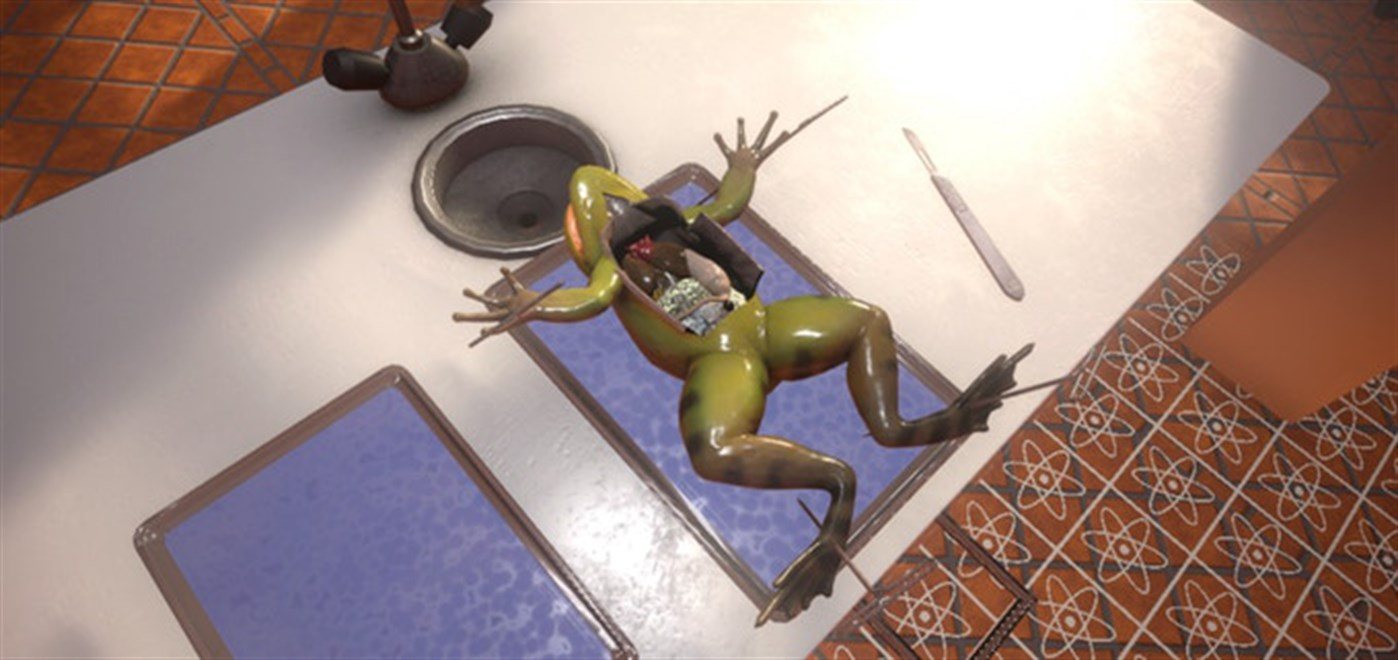
\includegraphics[scale=0.16]{Images/Estado del arte/frogDisection1.jpeg}\\
    \end{minipage}
    \begin{minipage}{0.5\textwidth}
        \centering
        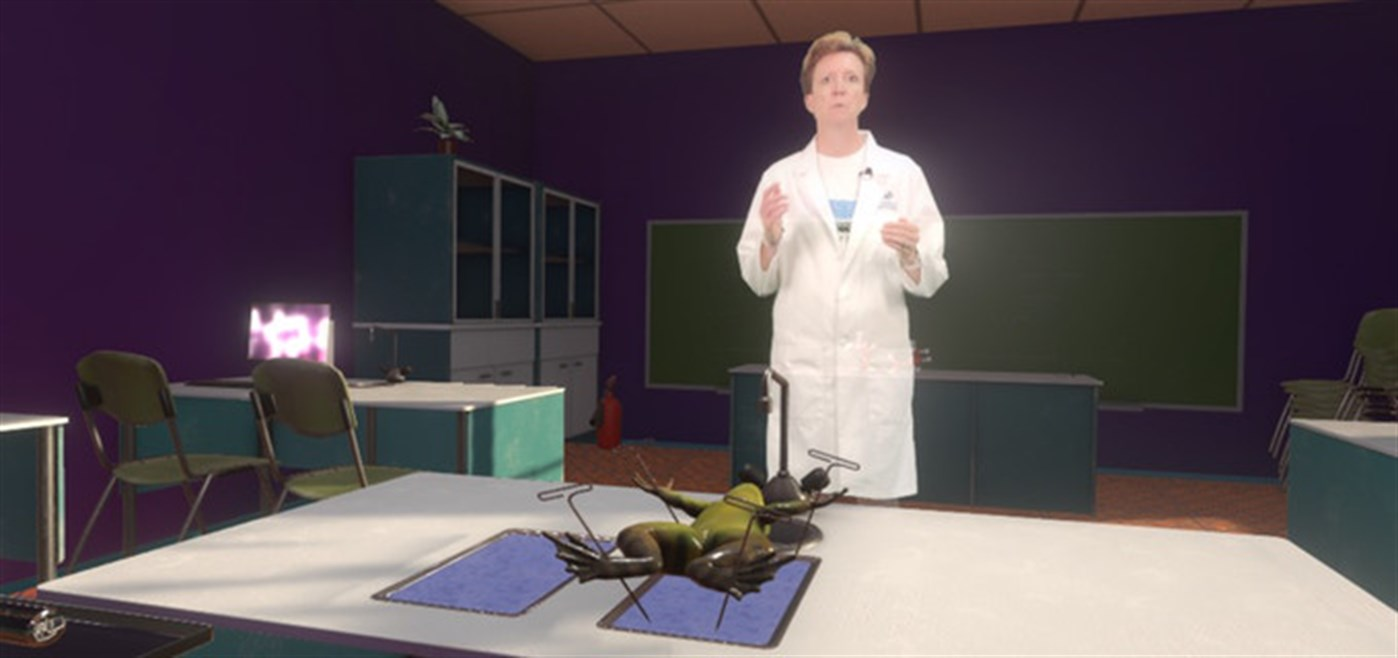
\includegraphics[scale=0.16]{Images/Estado del arte/frogDisection2.jpeg}\\
    \end{minipage}\\
    \caption[VR Frog Dissection: Ribbit-ing Discoveries]{\textit{VR Frog Dissection: Ribbit-ing Discoveries}\footnotemark.}
    \label{fig:vrfrogdissectioncapturas}
\end{figure}

\footnotetext{VR Frog Dissection: Ribbit-ing Discoveries: \href{https://www.microsoft.com/es-es/p/vr-frog-dissection-ribbit-ing-discoveries/9mvjk426cbt1?CustomerIntent=Consumer&activetab=pivot\%3Aoverviewtab#}{\nolinkurl{https://www.microsoft.com/es-es/p/vr-frog-dissection}}}

Otras de las muchas experiencias que nos ofrece la plataforma \textit{Windows Mixed Reality} son \textit{HoloTour} (una combinación de vídeo de 360 grados, sonido espacial y paisajes holográficos) o la aplicación de navegación 3D a través del cuerpo humano llamada \textit{Holo-Human}. Se puede usar esta experiencia de forma colaborativa para descubrir la anatomía de un cuerpo humano (figura \ref{fig:capturaHoloHuman}).

\begin{figure}[H]
    \centering
    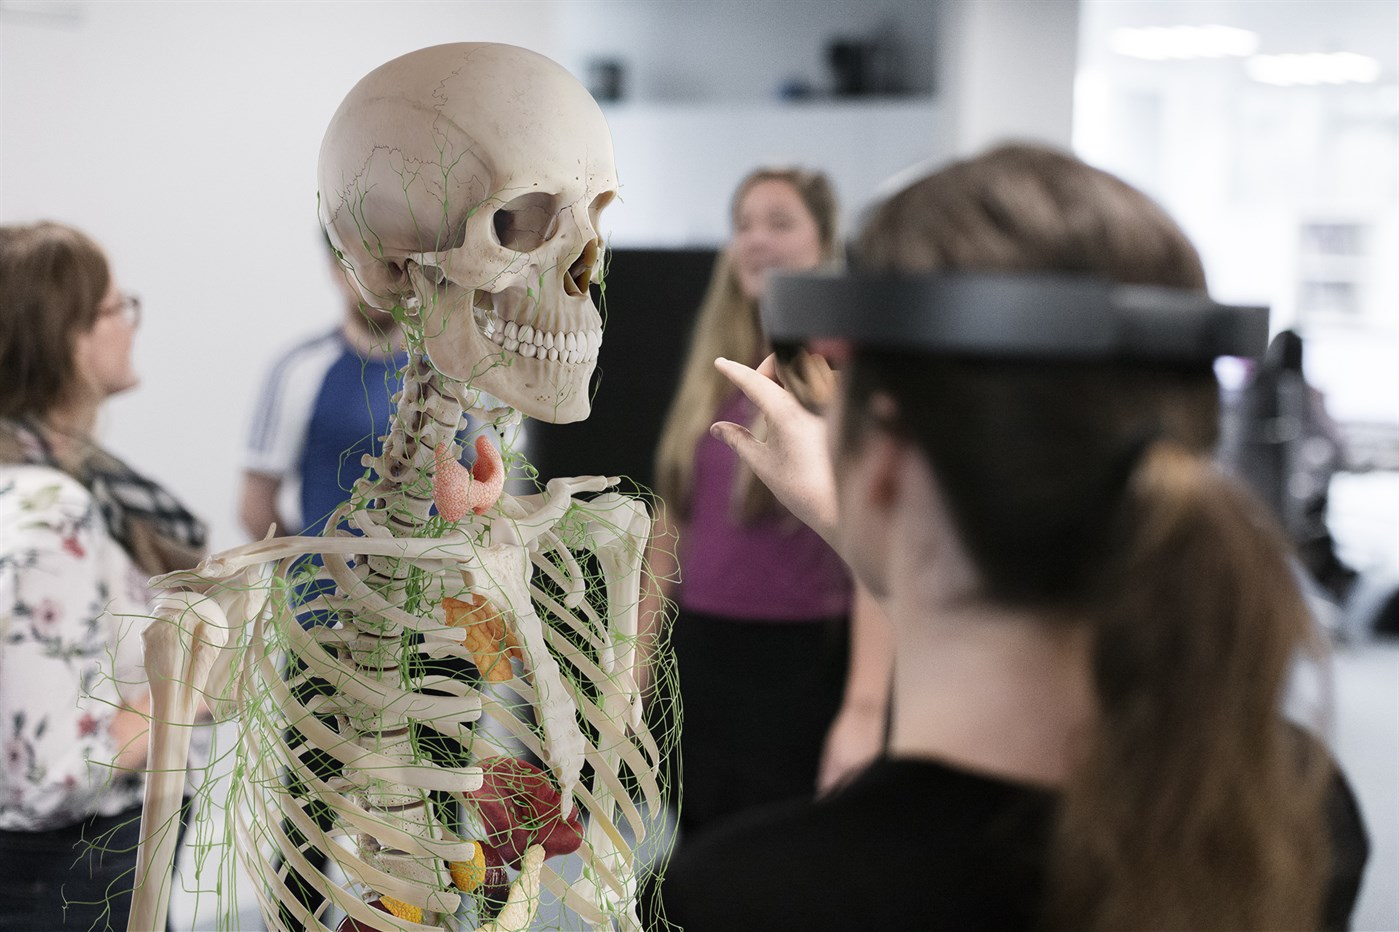
\includegraphics[scale=0.18]{Images/Estado del arte/holohuman.jpeg}
    \caption[Uso de la aplicación \textit{Holo-Human}]{Uso de la aplicación \textit{Holo-Human}\footnotemark.}
    \label{fig:capturaHoloHuman}
\end{figure}

\footnotetext{\textit{Holo-Human}: \href{https://www.microsoft.com/es-es/p/holo-human/9pggbknrbckj?CustomerIntent=Consumer&activetab=pivot\%3Aoverviewtab#}{\nolinkurl{https://www.microsoft.com/es-es/p/holo-human}}}

%https://www.microsoft.com/es-es/p/holo-human/9pggbknrbckj?CustomerIntent=Consumer&activetab=pivot%3Aoverviewtab#

